%tex file for ISCIE International Symposium on 
%            Stochastic Systems Theory and Its Applications
%
%

%latex209
%\documentstyle[sss,epsfig]{article}

%latex2e
\documentclass[a4paper]{article}
\usepackage{latexsym}
\usepackage{sss}
\usepackage{graphicsx} % for pdf, bitmapped graphics files
\usepackage{epsfig} % for postscript graphics files
\usepackage{amsmath}

\begin{document}
\date{}
\title{\LARGE{\bf
Direction Control of Moving Vehicle using Dual RTK-GNSS and Kalman Filter}
}
\author{
Shingo Kaminokado \\
Dept. of Computer Science and Engineering, The University of Aizu\\
Turuga, Ikki-machi, Aizuwakamatsu City, Fukushima, 965-8580 \\
\\E-mail: \texttt{m5211128@u-aizu.ac.jp}
}

\maketitle
\thispagestyle{empty}
%ABSTRACT
\abstract{
We have been investing a weeding robot. The robot estimates its position with 
Global Navigation Satellite System(GNSS) but includes errors, which are around 
a few meters, when it does single positioning. The direction of the robot deviates 
a lot as it is based on location information. Hence by using the more accurate Real 
Time Kinematic GNSS (RTK-GNSS), the positional accuracy improved. However, since 
the direction of the robot was estimated from the difference with the position of 
the previous robot, it was difficult to estimate the direction while posing. Therefore, 
we presumed self-position with two single frequency RTK-GNSS receivers which become 
to be available recently and are economically friendly. By setting the normal vector
calculated from the left and right position information with two modules as 
the direction of the robot, it made it possible to estimate the direction not 
only while running but also posing. Moreover, we will tackle construction of position 
estimation system with Kalman filter.
}


\section{Introduction}
Our research group has been developed a small weeding robot\cite{aigamo}. This robot weeds automatically in paddy fields.
It is important for the robot to know the self-position because it moves in a vast environment. To know the self-position, 
some researchers use camera\cite{camera-relate} or beacon\cite{beacon-relate}. 
However, these devices easily affected by disturbance such as weather, so it is difficult to apply to our robot.
Therefore, we adopt Global Navigation Satellite System(GNSS) to obtain self-position of the robot.
Conventionally, robots obtain self-position by single-positioning method.
However, position errors and orientation errors are greatly increase.
Therefore, we adopt Real Time Kinematic-GNSS (RTK-GNSS) for higher accuracy.
GNSS modules mainly receive two kinds of carries.
Dual frequency receivers are expensive and large, so we can not mount our robot.
On the other hand, the number of satellites has increased by multi-GNSS technology in recent years. As a result, cheap and compact modules that can acquire one frequency carrier have been on the market.
Therefore, we adopt these modules.
We installed two modules on the both side of the robot because it is difficult to estimate the orientation of the robot using only one module.
In this research, we propose a more accurate self-localization system by introducing the Kalman filter into our positioning system.
We verify our proposed method by Matlab.

\section{カルマンフィルタの説明}
この章では提案するカルマンフィルタのモデルを説明をする.
本研究ではアイガモロボットを対象としており,このロボットは2次元平面上を移動する.カルマンフィルタの予測フェーズ
\begin{align}
    \hat{x}_{t+ \Delta t|t} &= F_{t} \hat{x}_{t} + B_{t} u_{t} \nonumber \\
                            &= \hat{x}_{t} + B_{t} u_{t}
    \label{eq:1}
\end{align}
%
%
\begin{align}
    \hat{P}_{t+ \Delta t|t} &= F_{t} P_{t|t} F_{t}^{T} + Q \nonumber \\
                            &= P_{t|t} + Q
    \label{eq:2}
\end{align}
%
%
\begin{equation}
    \begin{bmatrix}
    \hat{x}_{t+ \Delta t|t} \\
    \hat{y}_{t+ \Delta t|t} \\
    \hat{\theta}_{t+ \Delta t|t}
    \end{bmatrix} 
    =
    \begin{bmatrix}
        \hat{x}_{t|t} \\
        \hat{y}_{t|t} \\
        \hat{\theta}_{t|t}
    \end{bmatrix} 
    +
    \begin{bmatrix}
        \Delta t cos\hat{\theta}_{t|t} &0 \\
        \Delta t sin\hat{\theta}_{t|t} &0 \\
        0                              &{\Delta}t
    \end{bmatrix}
    \begin{bmatrix}
        v_{t} \\
        \omega_{t}
    \end{bmatrix}
    \label{eq:3} 
\end{equation}
%
%
\begin{equation}
    e_{t} = \hat{x}_{t} - x_{t} =
    \begin{bmatrix}
        \hat{x}_{t} - x_{t} \\
        \hat{y}_{t} - y_{t} \\
        \hat{\theta}_{t} - \theta_{t}
    \end{bmatrix}
    \label{eq:4}
\end{equation}
%
%

\begin{equation}
    P_{t|t} = E
    \begin{pmatrix}
        e_{t} e_{t}^{T}
    \end{pmatrix}
    \label{eq:5}
\end{equation}
%
%
\begin{equation}
    \begin{split}
    \begin{bmatrix}
    \sigma_{xx,t|t+\Delta t} &\sigma_{xy,t|t+\Delta t} &\sigma_{xz,t|t+\Delta t} \\
    \sigma_{yx,t|t+\Delta t} &\sigma_{yy,t|t+\Delta t} &\sigma_{yz,t|t+\Delta t} \\
    \sigma_{zx,t|t+\Delta t} &\sigma_{zy,t|t+\Delta t} &\sigma_{zz,t|t+\Delta t} 
    \end{bmatrix} \\
    = 
    \begin{bmatrix}
        \sigma_{xx,t|t} &\sigma_{xy,t|t} &\sigma_{xz,t|t} \\
        \sigma_{yx,t|t} &\sigma_{yy,t|t} &\sigma_{yz,t|t} \\
        \sigma_{zx,t|t} &\sigma_{zy,t|t} &\sigma_{zz,t|t}
    \end{bmatrix} 
    +
    \begin{bmatrix}
        q_{x}^{2} &0         &0 \\
        0         &q_{y}^{2} &0 \\
        0         &0         &q_{\theta}^{2}
    \end{bmatrix}
\end{split}
    \label{eq:6} 
\end{equation}


\section{カルマンフィルタに用いる分散の取得実験}

Regarding the styles of your manuscript, please conform to the following 
%instructions. 

\subsection{Title}
\subsection{Author's Names and Address}
\subsection{Headings}
\subsection{Figures and Tables} 


\subsection{References}


\subsection{Page Numbers}



\section{Simulation using Kalman filter}
%先行研究より、我々の測位システムの位置と向きの分散共分散行列を算出した.
%これを用いてDual RTK-GNSSにおけるカルマンフィルターの優位性についてシミュレーションする.
%
%
%
%
%
%

\subsection{Result}
\begin{figure}
\centerline{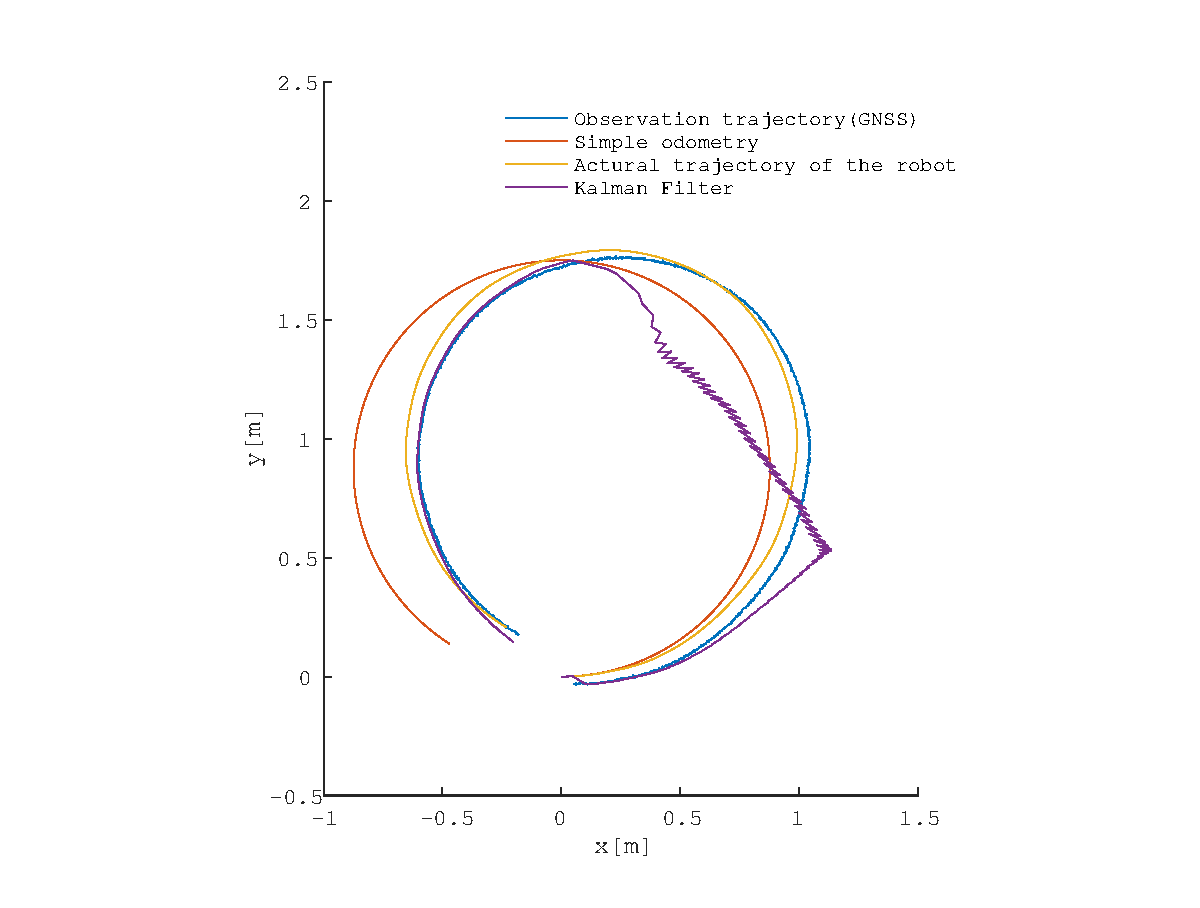
\epsfig{file=process_noise_S.eps,width=100mm}}
\caption{Large Process noise}
\centerline{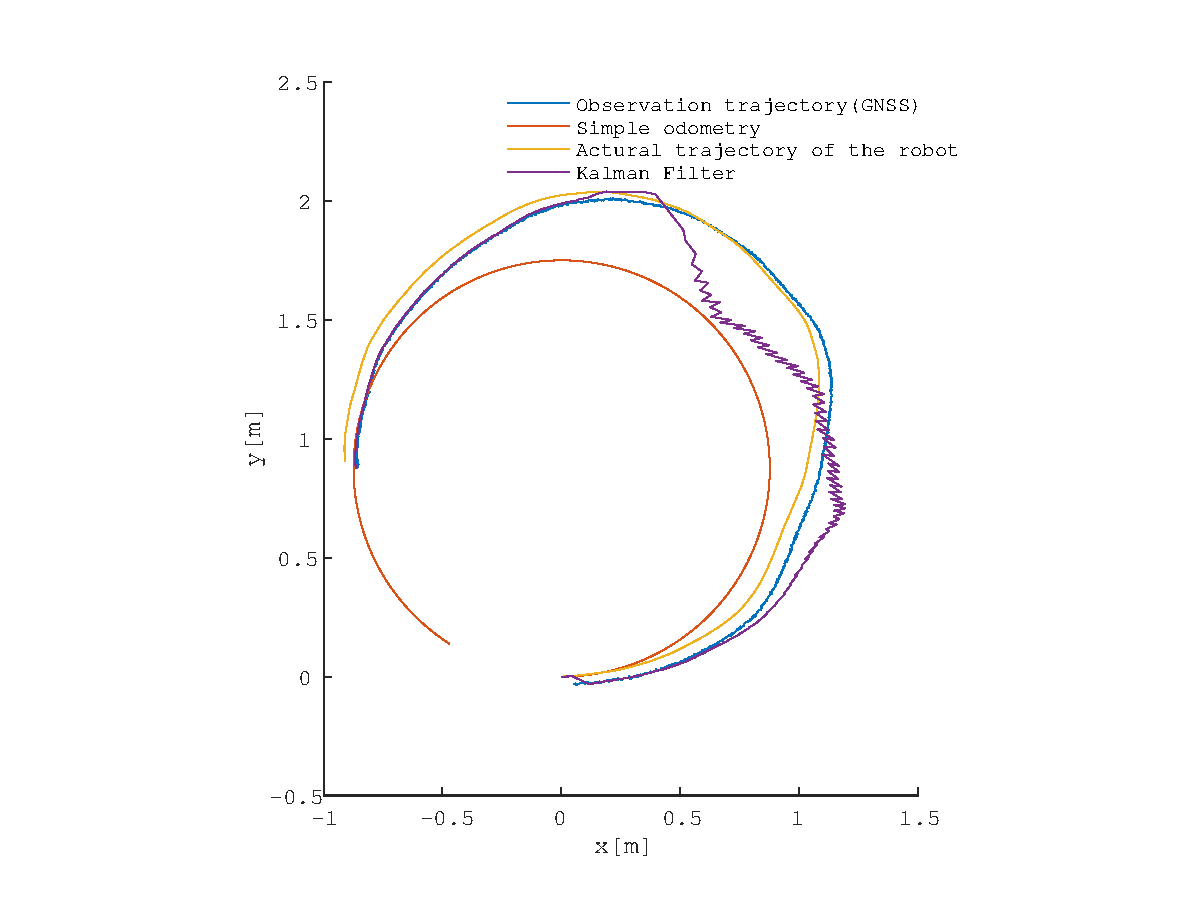
\epsfig{file=process_noise_M.eps,width=100mm}}
\caption{Middle Process noise}
\centerline{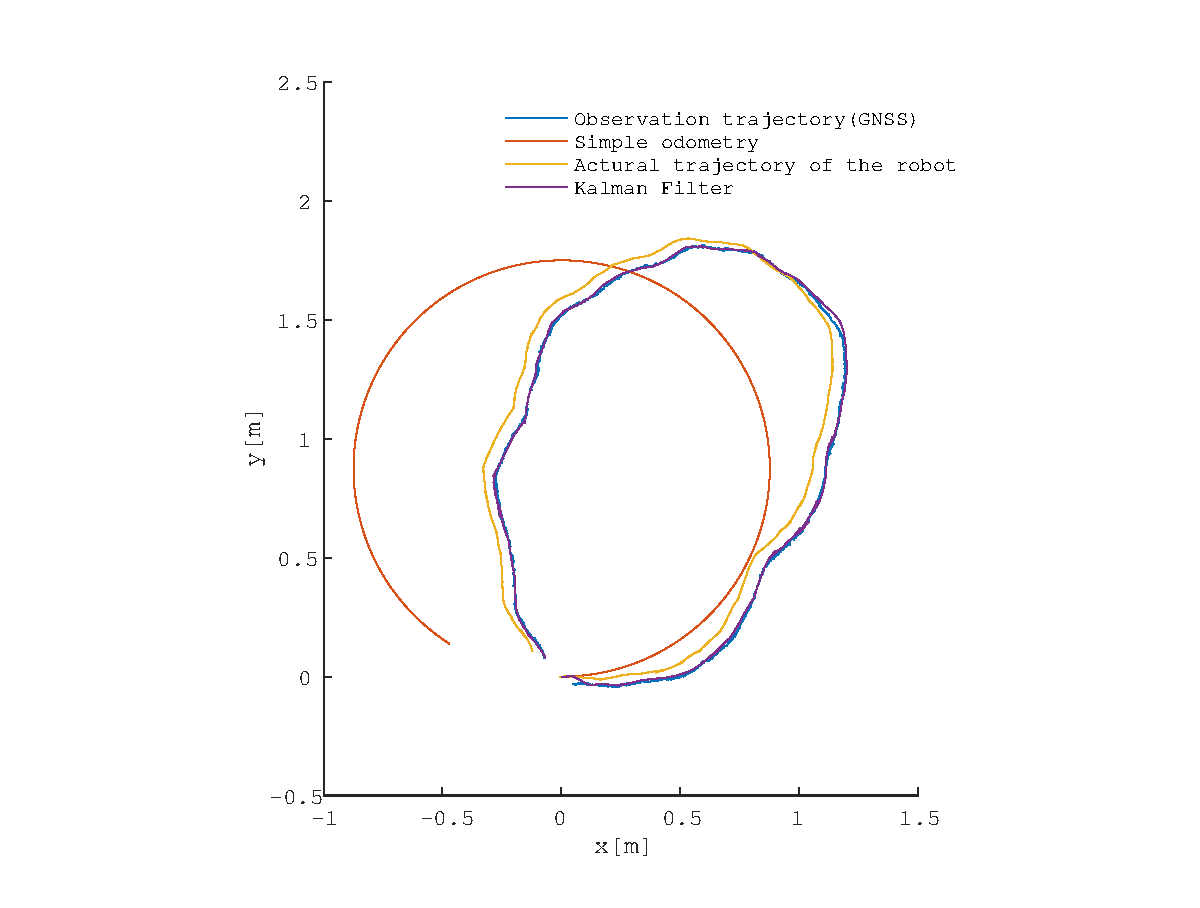
\epsfig{file=process_noise_L.eps,width=100mm}}
\caption{Small process noise}
\end{figure}
\subsection{Disucussion}


\section{Conclusions}

\begin{thebibliography}{99}
\bibitem{aigamo}
M. Taku, O. Yoshiaki, O. Jun, N. Keita and N. Keitaro:
Mechanism of generating drawbar pull of rod wheel on loose soil,
{\it 22rd International Symposium on Artificial Life and Robotics.(AROB)}, Vol.22, No.4, 2017.
\bibitem{camera-relate}
S.Shotaro, H. Zhencheng and F. Thomas:
Tracking ofFeatUre PointsforVisualSLAM with MultipleCameras
{\it The Institude of Image Information and Television Engineers}
\bibitem{beacon-relate}
Z. Fang, L. Deng, Y. Ou and X. Wu:
A tracking robot based on wireless beacon
{\it International Conference on Intelligent Robotics and Applications}, pp.191-202, 2010.
\bibitem{gnss}
H. J. Christopher and C. Eric:
Evolution of the global navigation satellitesystem (gnss),
{\it Proceedings of the IEEE}, Vol.96, No.12, pp.1902-1917, 2008.
\bibitem{rtk-gps}
K. Michio. N. Noboru, I. Kazunobu and T. Hideo: 
Field Mobile Robot navigated by RTK-GPS and FOG, 
{\it Journal of the Japanese Society of Agricultural Machinery}, Vol.63, No.5, pp.74-79, 2001.(in Japanese)
\bibitem{auto-weeding}
S. Masahiro, N. Yoshisada, T. Katsuhiko and K. Kyou: 
{\it Journal of the Japanese Society of Agricultural Machinery}, Vol.72, No.3, pp.276-282, 2010.(in Japanese)
\bibitem{reach rs} 
Emlid Reach RS, https://docs.emlid.com/eachrs/

\bibitem{reach} 
Emlid Reach, https://docs.emlid.com/each/
\end{thebibliography}
\end{document}

% end of sss10.tex
